\documentclass[oneside, landscape, twocolumn, a4wide, 9pt]{scrartcl}
\usepackage{savetrees}
\usepackage{bera}
\usepackage[brazilian]{babel}
\usepackage[utf8x]{inputenc}
\usepackage{epsfig}
\usepackage{amsmath}
\usepackage{amssymb}
\usepackage{amsthm}
\usepackage{graphicx}
\usepackage{pstricks}
\usepackage{cancel}
\usepackage{tocloft}
\usepackage{titlesec}
\usepackage{fancyvrb}
\usepackage{pdfpages}
\usepackage{fancyhdr}

\setlength{\columnsep}{.25in}
\setlength{\columnseprule}{.25pt}
\parindent=0in

\setcounter{tocdepth}{1}

\renewcommand{\cftbeforesecskip}{0cm}

\fvset{fontsize=\small}

\titleformat{\section}
{\titlerule
\vspace{0.1cm}%
\normalfont\bf\itshape}
{\thesection.}{.5em}{}

\DefineShortVerb{\|}

\pagestyle{fancyplain}
\renewcommand{\headrulewidth}{.25pt}
\fancyhf{}
\lhead{\huge\sf ITA - Carteado}
\chead{}
\rhead{\huge\sf\thepage}
\lfoot{}
\cfoot{}
\rfoot{}

\begin{document}
\begin{center}
{\bf
  LIBRARY\\
  EQUIPE ITA-CARTEADO\\}
\end{center}
\vspace{-0.5cm}
\tableofcontents
\thispagestyle{fancyplain}

\section{Codigos de início de prova}
\subsection{Makefile}
\VerbatimInput{textMakefile.txt}
\subsection{modelo.cpp}
\VerbatimInput{modelo.cpp}
\subsection{struct.sh}
\VerbatimInput{struct.sh}

\section{Itens Importantes}
\subsection{Antes de começar}
\begin{itemize}
\item Reler a estratégia de prova algumas vezes
\item Reler a lista de algoritmos no bizuário
\end{itemize}
\subsection{Resolvendo um problema}
\begin{itemize}
\item LAPDED - Leia a PORRA do enunciado direito!
\item Faça as contas! Limites de arrays e cuidado com overflows
\item Peça as clarifications antes
\end{itemize}
\subsection{Debugando um problema}
\begin{itemize}
\item WA/RE, não sabe por quê e mais de 30min sem idéia? Implementa de novo
\item Bugs e casos extremos: criar casos de teste, sempre
\item Compiler Error em ambientes toscos: busca binária em casos extremos
\end{itemize}
\subsubsection{Bugs do milênio}
\begin{itemize}
\item Verificar overflows, ver se o $\infty$ é tão infinito quanto parece
\item Doubles: igualdade com tolerância
\item Igualdade dentro de |if|
\item |C-w C-y|? Errou algo.
\item Tamanho de vetores
\item |long long a = 1 << 40;| $\Longrightarrow$ |long long a = 1ll << 40;| %>>>>
\item Variáveis com nome min,max
\item Inicialização de variáveis
\item Casos extremos, muito pequenos ou muito grandes
\item Self-loops e multiarestas em grafos
\item Otimização de casos específicos
\item Imprecisão ao subtrair números quase iguais
\item Resto de divisão com números negativos
\end{itemize}

\section{Estratégia}
\subsection{300 minutos - Início}
\begin{itemize}
\item Digitar |Makefile|, |modelo.cpp| e |struct.sh|
\item Criar os fontes modelo usando |struct.sh problema1 ... problemaN|
\item Enquanto isso (ou enquanto o primeiro problema estiver sendo
  resolvido), outras duas pessoas dividem os problemas e começam a
  ler, anotando no quadro ordem de resolução e idéias
  preliminares. Não ter medo de colocar infinito no problema.
\item Ler o máximo de problemas possível.
\item Na dúvida, olhar os balões e o scoreboard.
\end{itemize}
\subsection{200 minutos - Meio}
\begin{itemize}
\item Todos já devem ter lido todos os problemas não resolvidos da prova
\item Limite de questões em paralelo: {\bf 2 ou 3}
\item Logo que mandar o problema, mande imprimir código e saída (com debug)
\item WA/RE, não sabe por quê, 30+ min sem idéia? Pense em reimplementar.
\item Na dúvida, olhar os balões e o scoreboard.
\end{itemize}
\subsection{100 minutos - Começo do fim}
\begin{itemize}
\item Limite de questões em paralelo: {\bf 1 ou 2}
\item Olhar os baloẽs e o scoreboard - escolha dos problemas difíceis
\item Equipe mais unida
\end{itemize}
\subsection{15 minutos - Juízes calados}
\begin{itemize}
\item Mexer um pouco e mandar. Tirar debug. Pensar só depois em mais casos de teste.
\end{itemize}

\section{Geometria (números inteiros)}
\VerbatimInput{geometria-inteiros.cpp}

\section{Geometria (ponto flutuante)}
\VerbatimInput{geometria-doubles.cpp}

\section{Teoria dos Números}
\VerbatimInput{ntheory.cpp}

\section{Garfos}
\VerbatimInput{grafos.cpp}

\section{BigNum}
\VerbatimInput{bignum.cpp}

\section{Álgebra Linear}
\VerbatimInput{alglin.cpp}

\section{Strings}
\VerbatimInput{strings.cpp}

\section{Binary Indexed Tree}
\VerbatimInput{bit.cpp}

\section{Interval Tree}
\VerbatimInput{intervaltree.cpp}

\section{Problemas}
\VerbatimInput{problemas.cpp}

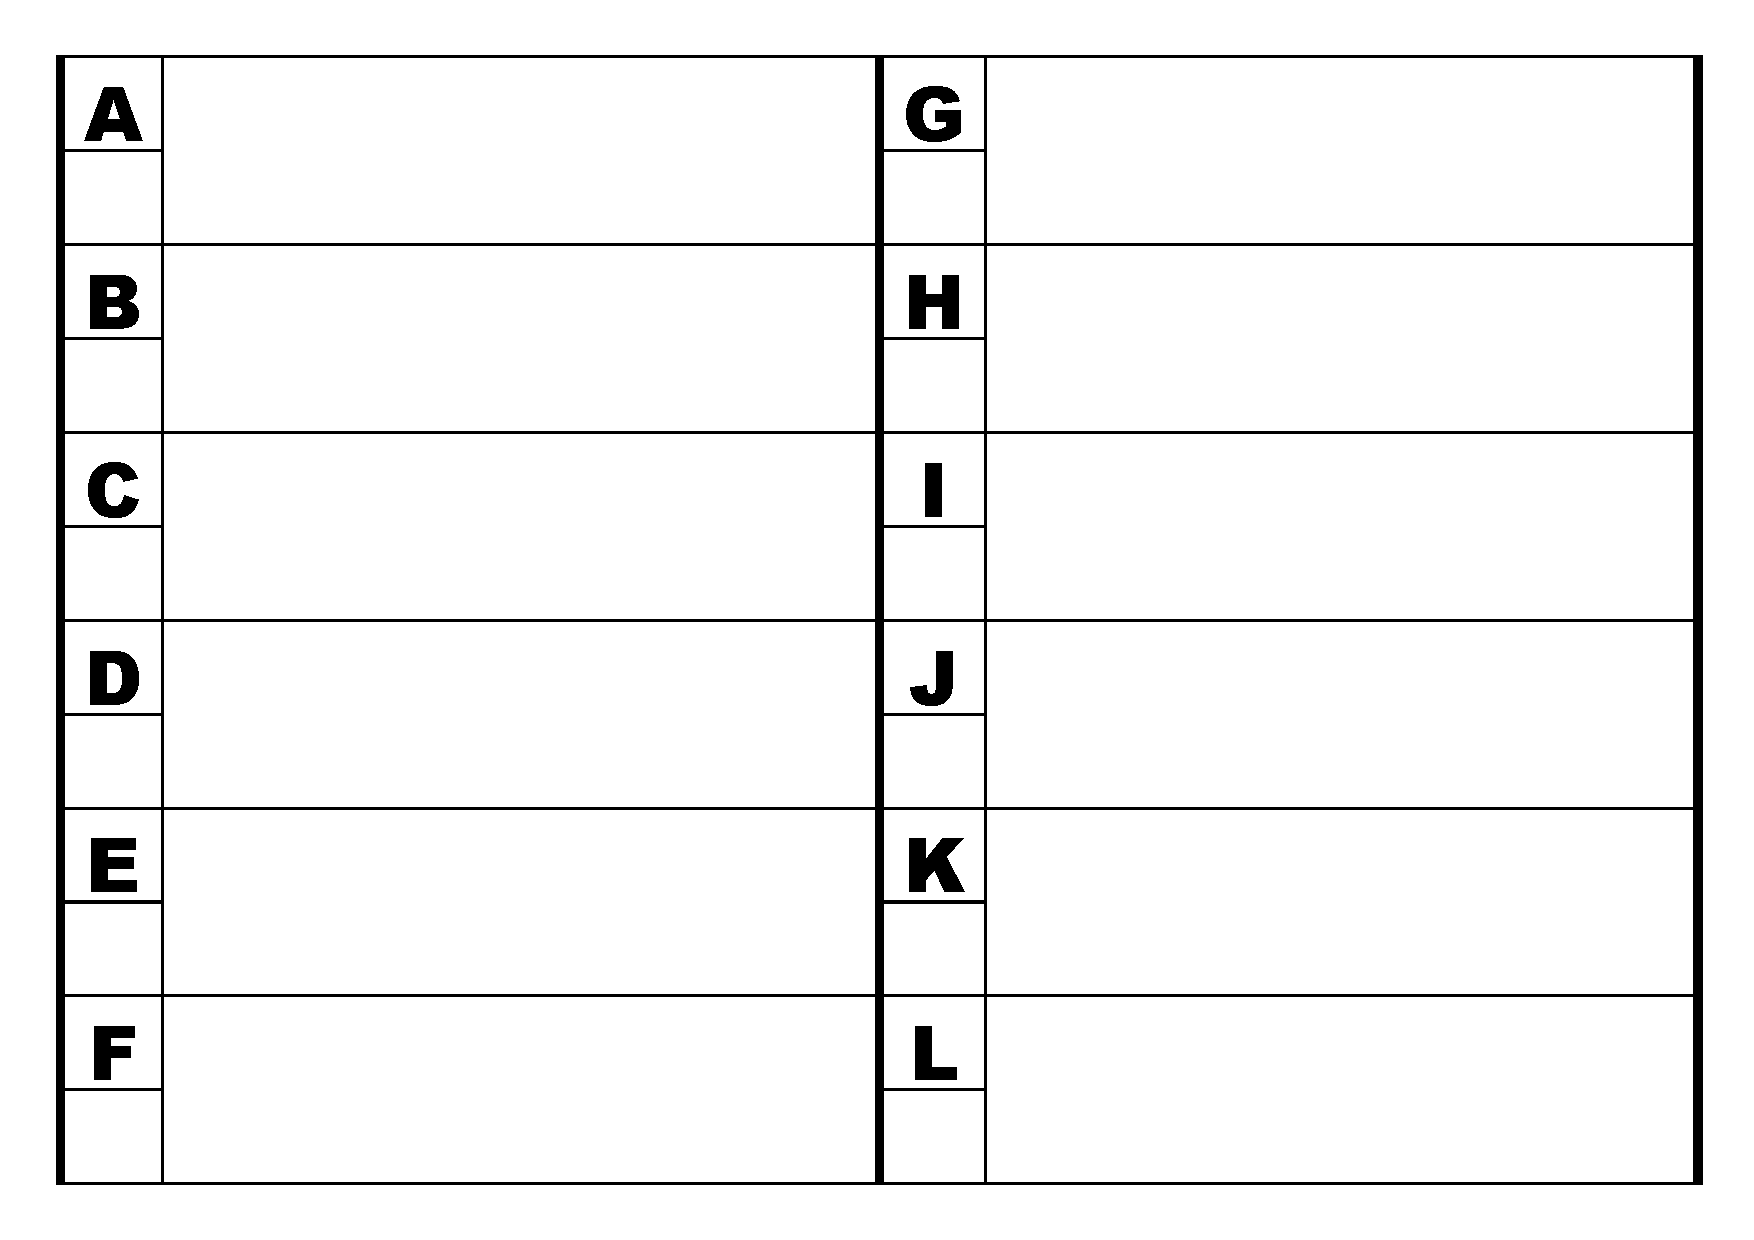
\includepdf[pages=1]{status-v2}

\end{document}

